\documentclass[12pt]{article}
\usepackage{comment}
\usepackage[utf8]{inputenc}
\usepackage{xspace}
\usepackage{gastex}
\usepackage{amsmath}
\usepackage{amssymb}
\usepackage{wrapfig}
\usepackage{tikz}
\usepackage{float}
\usepackage{pgfplots}
\usepackage{booktabs} % For \toprule, \midrule and \bottomrule
\usepackage{pgfplotstable} % Generates table from .csvi
\usepackage{csquotes}
\usepackage{graphicx}
\usepackage{amsmath}
\usepackage{multicol}
\usepackage{tgtermes} % times font
\usepackage[shortlabels]{enumitem}
\usepackage{parskip}

\pagestyle{empty}
\textwidth      165mm
\textheight     252mm
\topmargin      -18mm
\oddsidemargin  -2mm
\evensidemargin -2mm
% \renewcommand{\baselinestretch}{0.96}
\newcommand{\impl}{\mathbin{\Rightarrow}}
\newcommand{\biim}{\mathbin{\Leftrightarrow}}
\newcommand{\id}[1]{\mbox{\textit{#1}}}
\newcommand{\tuple}[1]{\langle #1 \rangle}
\newcommand{\ma}{\mathsf{a}}
\newcommand{\mb}{\mathsf{b}}
\newcommand{\mc}{\mathsf{c}}
\newcommand{\md}{\mathsf{d}}
\newcommand{\nat}{\mathbb{N}}
\newcommand{\intg}{\mathbb{Z}}

\newcounter{question}
\newcommand{\question}[1]{
    \stepcounter{question}
    \thequestion. #1 \hfill
}

\newcommand{\revision}[1]{
    \stepcounter{question}
    \thequestion. #1* \hfill
}



\begin{document}
\topskip0pt
\begin{center}
    {\sc The University of Melbourne
        \\
        School of Computing and Information Systems
        \\
    COMP90020 Distributed Algorithms}
    \bigskip \\
    {\Large\bf Tutorial Week 7: Multicast}
    \bigskip \\
\end{center}

\section*{Notes}



\section*{Exercises}

\setcounter{question}{29}

\question{How, if at all, should the definitions of integrity, agreement and validity for reliable multicast change for the case of open groups?}

\question{Explain why reversing the order of the lines \begin{center}\textit{R-Deliver m} \\ \textit{if ($q \not = p$) then B-multicast(g,m) end if} \end{center} \\ as shown in this algorithm, would make the algorithm no longer satisfy uniform agreement. Does the reliable multicast algorithm based on IP multicast satisfy uniform agreement?}

\question{Show that the FIFO-ordered multicast algorithm does not work for overlapping groups, by considering two messages sent from the same source to two overlapping groups, and considering a process in the intersection of those groups. Adapt the protocol to work for this case. Hint: processes should include with their messages the latest sequence numbers of messages sent to all groups.}

\question{In a group, there are eight members, of which at most one can crash at any time.  You have no idea about which process can crash. The topology is a completely connected network.}

\begin{enumerate}[(a)]
    \item In the worst case, what is the samllest number of messages requireed to gaurantee reliable atomic multicast from a given process to the entire group?
    \item How does this change if up to four members can crash at any time?
\end{enumerate}


\question{Show that, if the basic multicast that we use in the algorithm of the attached figure is also FIFO-ordered, then the resultant totally-ordered multicast is also causally ordered. Is it the case that any multicast that is both FIFO-ordered and totally ordered is thereby causally ordered?}

\begin{center}
    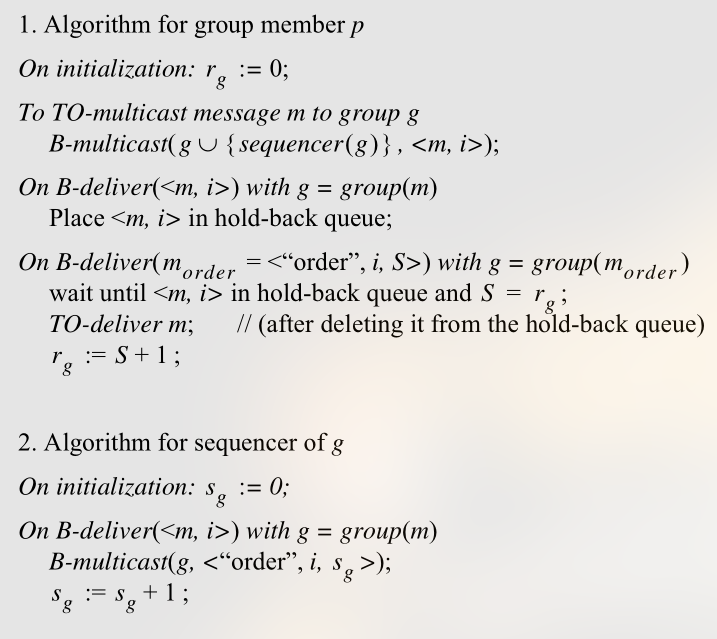
\includegraphics[scale=0.70]{multicast.png}
\end{center}

\question{Consider a multiparty game of quiz involving five teams. \begin{quote} Each team poses a question and a member of another team has to answer it. The team that answers the question first scores a point. If no team can answer a question within 30 s, then no one scores any point. The clocks are synchronized, so who answered first is decided by the time when the reply was posted. The teams can pose questions at any time and in no particular order. \end{quote} What kind of multicast is appropriate here?  }


\question{Consider an election in a state. The citizens cast their votes at the individual polling centers. At the end of the day when the poll closes, counting begins. Each count recorded at a center is multicast to all the other centers, so that all of them exactly know the latest count at any time when the counting is in progress. The interconnection topology of the network connecting the polling centers is a completely connected graph.*}

\begin{enumerate}[(a)]
    \item Assume that at any time failures can bring down some of the communication lines without creating a partition. What kind of multicast will guarantee that all centers are able to record every vote?
    \item Assume that communication failure partitioned the network for an hour. Apparently the counting must stop. What  would you recommend so that the progress of counting is not affected even if the network temporarily partitions?
\end{enumerate}

\end{document}
